%%%%%%%%%%%%%%%%%%%%%
% Experiments and Results %
%%%%%%%%%%%%%%%%%%%%%

This thesis aims to analyze the relationships between different road networks and road network similarity methods. In particular,  (1) the similarities between different road networks are determined, (2) similar road networks are clustered, (3) the correlations between the different network similarity methods used to identify the similarities between the different road networks are also determined, and (4) the similar methods are clustered. Figures \ref{fig:Road Network Similarity and Ranking} and \ref{fig:Road Network Similarity Method Correlation} show a high-level overview of the process. 

\begin{figure}[h]
\centering

\includegraphics[width=0.75\textwidth,center]{picture/network_ranking.png}
\caption[Road Network Similarity and Ranking]{Road Network Similarity and Ranking}
\label{fig:Road Network Similarity and Ranking}
\end{figure}

\begin{figure}[!ht]
\centering

\includegraphics[width=0.75\textwidth,center]{picture/ranking.png}
\caption[Road Network Similarity Method Correlation]{Road Network Similarity Method Correlation}
\label{fig:Road Network Similarity Method Correlation}
\end{figure}


\section{Grid Road Network Similarity Analysis}
This section describes the experiments to identify similar road networks with Grid patterns and structure, likewise groups of methods described in Chapter 3 that have similar behavior.

The problem to find road networks with similar structures and patterns is explicitly approached using network-similarity ranking[Soundarajan]. Firstly, a reference network Gr and a collection of comparison networks H1, H2,...., Hk are given. A network-similarity method is then used to calculate the similarity between Gr and each Hi. The data (similarity scores) for each comparison are normalized for uniformity before being used to create a dendrogram. This will cancel out the effects of outliers and ensure that the results have the same units. In Table 4.1 that shows the similarity score for each comparison, the normalization is accomplished by calculating Z scores for each similarity score in each column: z = (x mean)/std. As a result, the column mean is subtracted from each value in the column and then divided by the standard deviation. As a result, all the columns have the same mean and variance. The normed values indicate how many standard deviations any individual value deviates from the column mean. The hierarchical clustering algorithm can now be used in conjunction with the Ward variance minimization algorithm by combining the linkage function to generate the dendrogram. 

The District of Columbia (USA) is chosen as the reference network for the Grid road similarity analysis, and the methods are used to compare the other networks to the reference network and generate a numerical similarity score. The networks are then clustered in hierarchical order. The goal is to see if certain road networks are similar to the reference network's Grid pattern, which generates a dendrogram with road network patterns that are similar to the reference road network pattern. The results for this analysis are presented in Figure \ref{fig:Hierarchical Clustering Dendrogram for Grid Road Networking Similarity}.

\begin{figure}[!ht]
\centering
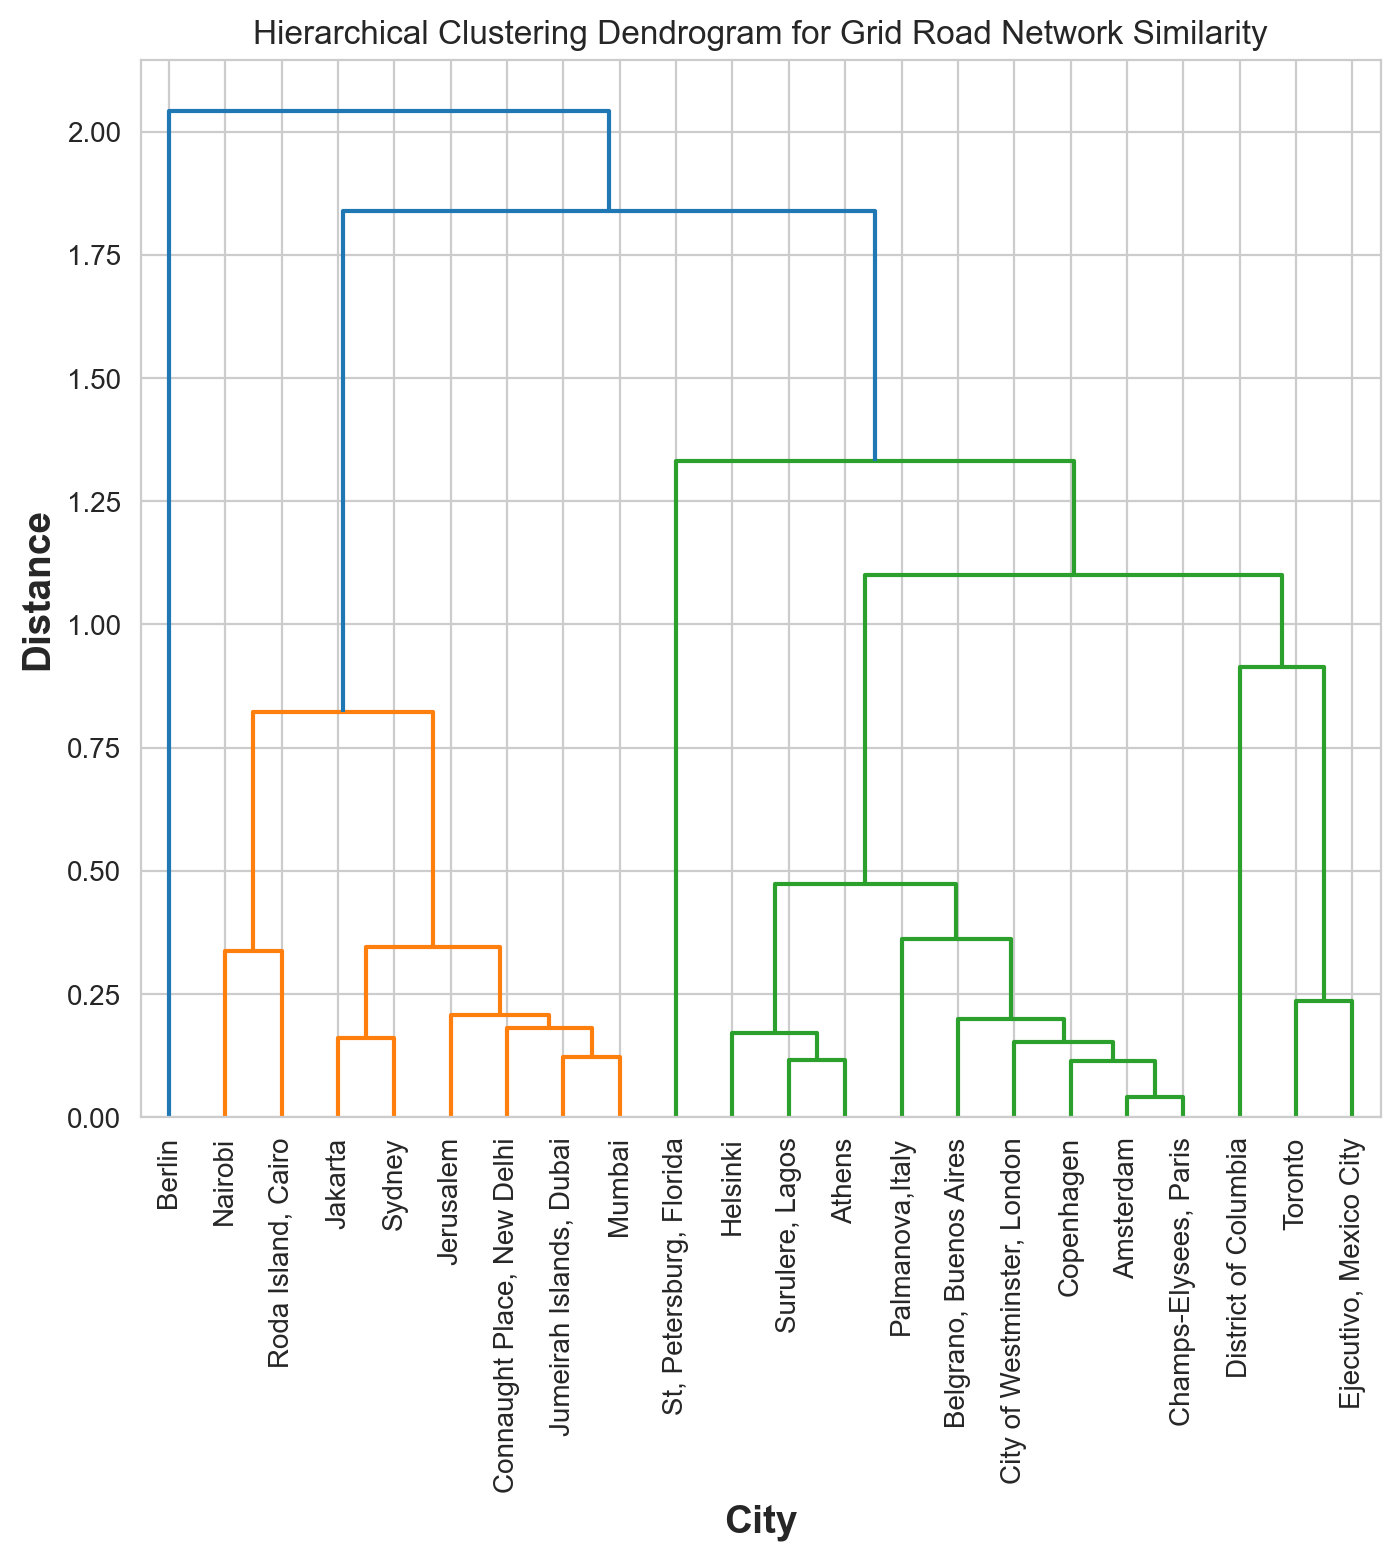
\includegraphics[width=0.75\textwidth,center]{picture/Grid/grid_dendrogram2.png}
\caption[Hierarchical Clustering Dendrogram for Grid Road Networking Similarity]{Hierarchical Clustering Dendrogram for Grid Road Networking Similarity}
\label{fig:Hierarchical Clustering Dendrogram for Grid Road Networking Similarity}
\end{figure}

Figure \ref{fig:Hierarchical Clustering Dendrogram for Grid Road Networking Similarity} presents the dendrogram obtained from the cluster analysis. The dendrogram  is interpreted using two criterias. First, a branch or cluster that includes the reference network. Second, the arrangement of the clusters which tells us the road networks that are most similar to each other, as the height of the cluster measured in distance, indicates how similar or different the road networks are from each other. The greater the distance, the greater the difference. 

For the first criteria, two major clusters (Green and Orange) can be observed from the dendrogram's structure except for the outlier; berlin road network (Blue). Looking at the green cluster, the road network for the cities Ejecutivo and Toronto lie near the reference network: District of Columbia (USA) in one adjacent cluster and are later grouped as a single cluster which indicates that this cities are the most pronounced grid-like structure similar to the reference network. 

Interpreting the dendrogram using the second criteria, the road networks for the cities Champs-Elysees, Paris and Amsterdam, Netherlands are said to be clustered first as they tend to have the cluster with the relatively shortest distance. Therefore they are the most similar than any other cluster of road networks at a higher level.

Initially, one will expect that the road networks within the green cluster should have similarities to the grid pattern of the reference network, likewise have clusters with the shortest distance, but by cross-checking with the similarity scores for each method included in the heatmap in figure \ref{fig:Heatmap showing the correlations for Grid Road Networks}, it is possible to identify the characteristics of each cluster and why certain clusters are grouped together.

\begin{figure}[!ht]
\centering
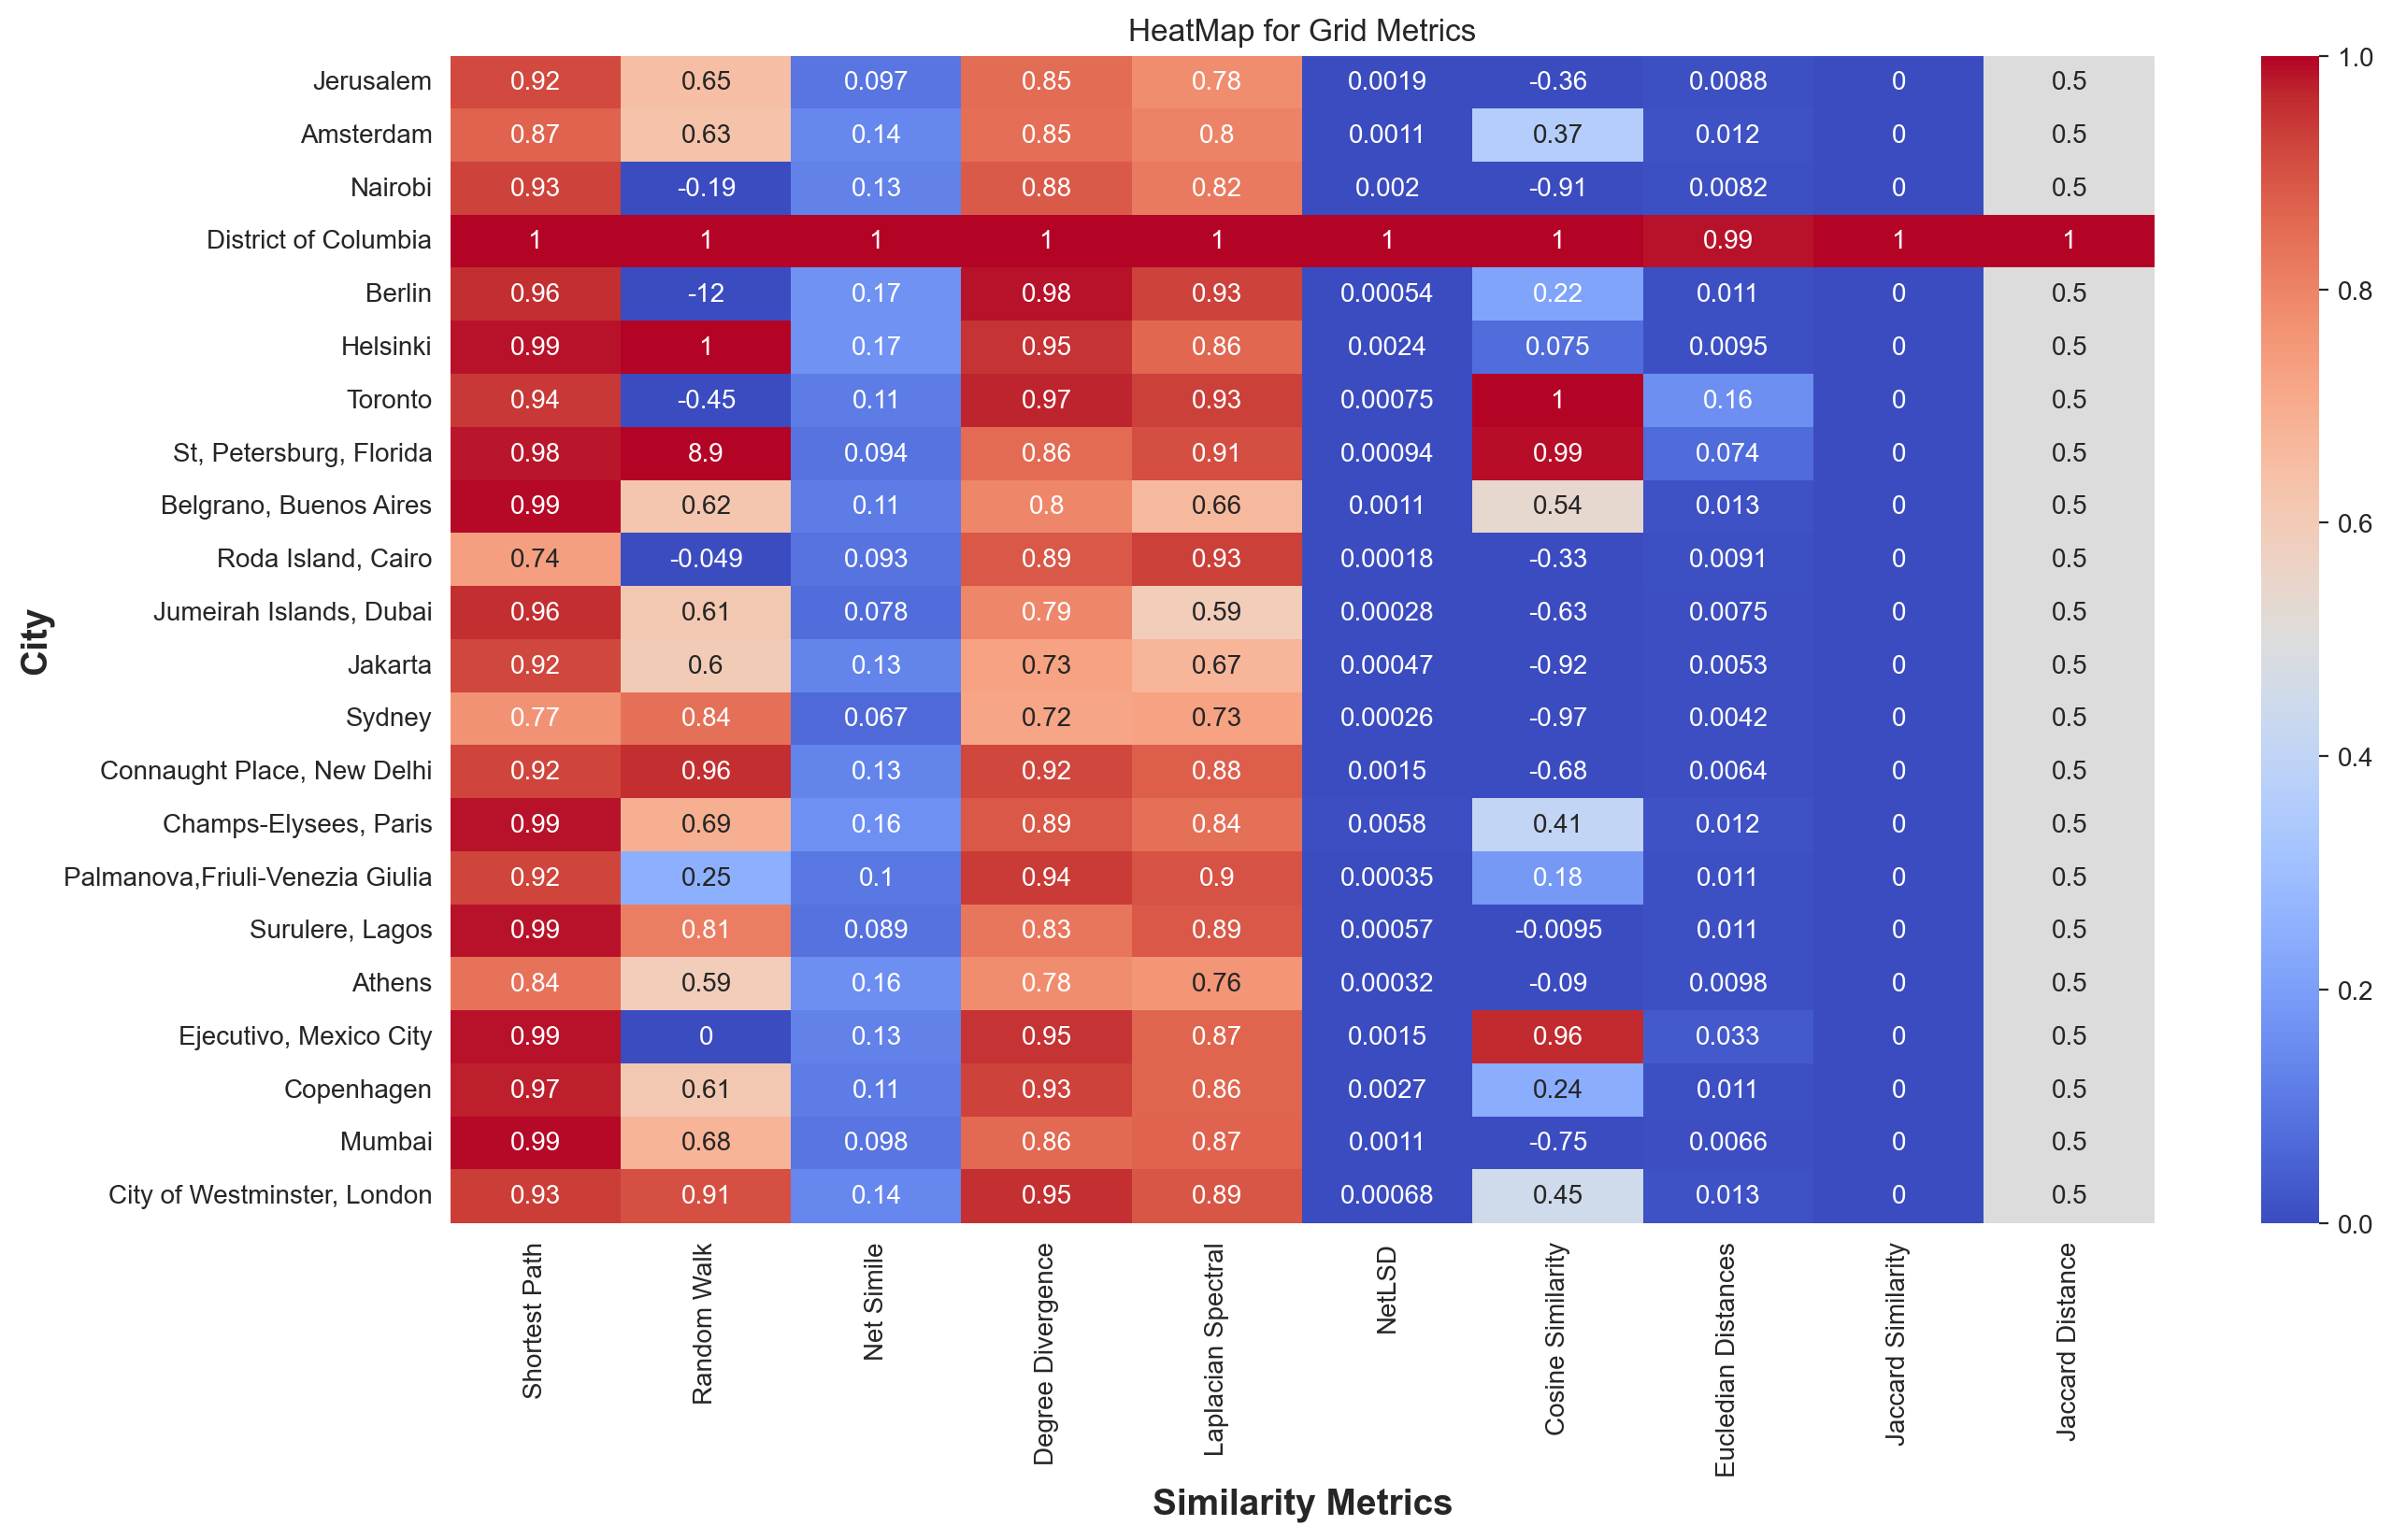
\includegraphics[width=0.85\textwidth,center]{picture/Grid/gridheatmap.png}
\caption[Heatmap showing the correlations for Grid Road Networks]{Heatmap showing the correlations between the road networks when the road network: District of Columbia was used as the reference network.}
\label{fig:Heatmap showing the correlations for Grid Road Networks}
\end{figure}


Furthermore, dendrograms only tell us a little bit about the similarities of road networks based on the clusers generated. The dendrogram clearly depicts a different picture, with some road networks grouped differently (see how the distribution of the road networks is mixed). For example, St. Petersburg, Florida, which is considered to be among the most similar to the reference network based on the similarity scores in figure \ref{fig:Heatmap showing the correlations for Grid Road Networks}, is later combined with the clusters of Ejecutivo, Toronto, and the District of Columbia (USA). As the dendrogram results are not intuitive, it is not suitable for interpreting the similarity results. Further analysis or another alternative to visualize the results of the similar scores is recommended.

In addition, dendrograms only tell us a bit in terms similarities of road networks based on the clusers generated. The dendrogram clearly shows a different picture, where some of the road networks are grouped differently (see how the distribution of the road networks is mixed). For example, St, Petersburg, Florida which from the similarity scores in figure \ref{fig:Heatmap showing the correlations for Grid Road Networks} considered to be amongst the most similar to the reference network is later put together with cluster of Ejecutivo, Toronto and the District of Columbia (USA). Further analysis is recommended or another alternative to visualize the results of the similar scores is recommended as the dendrogram results are not intuitive, thus making it not suitable for interpreting the similarity results.

To find methods that behave similarly, the pairwise Kendall-Tau distance between each pair of methods is calculated first, followed by a complete-linkage hierarchical clustering because it produces a dendrogram with many small clusters, which provides insight into which groups of methods are closely correlated.

\begin{figure}[!ht]
\centering
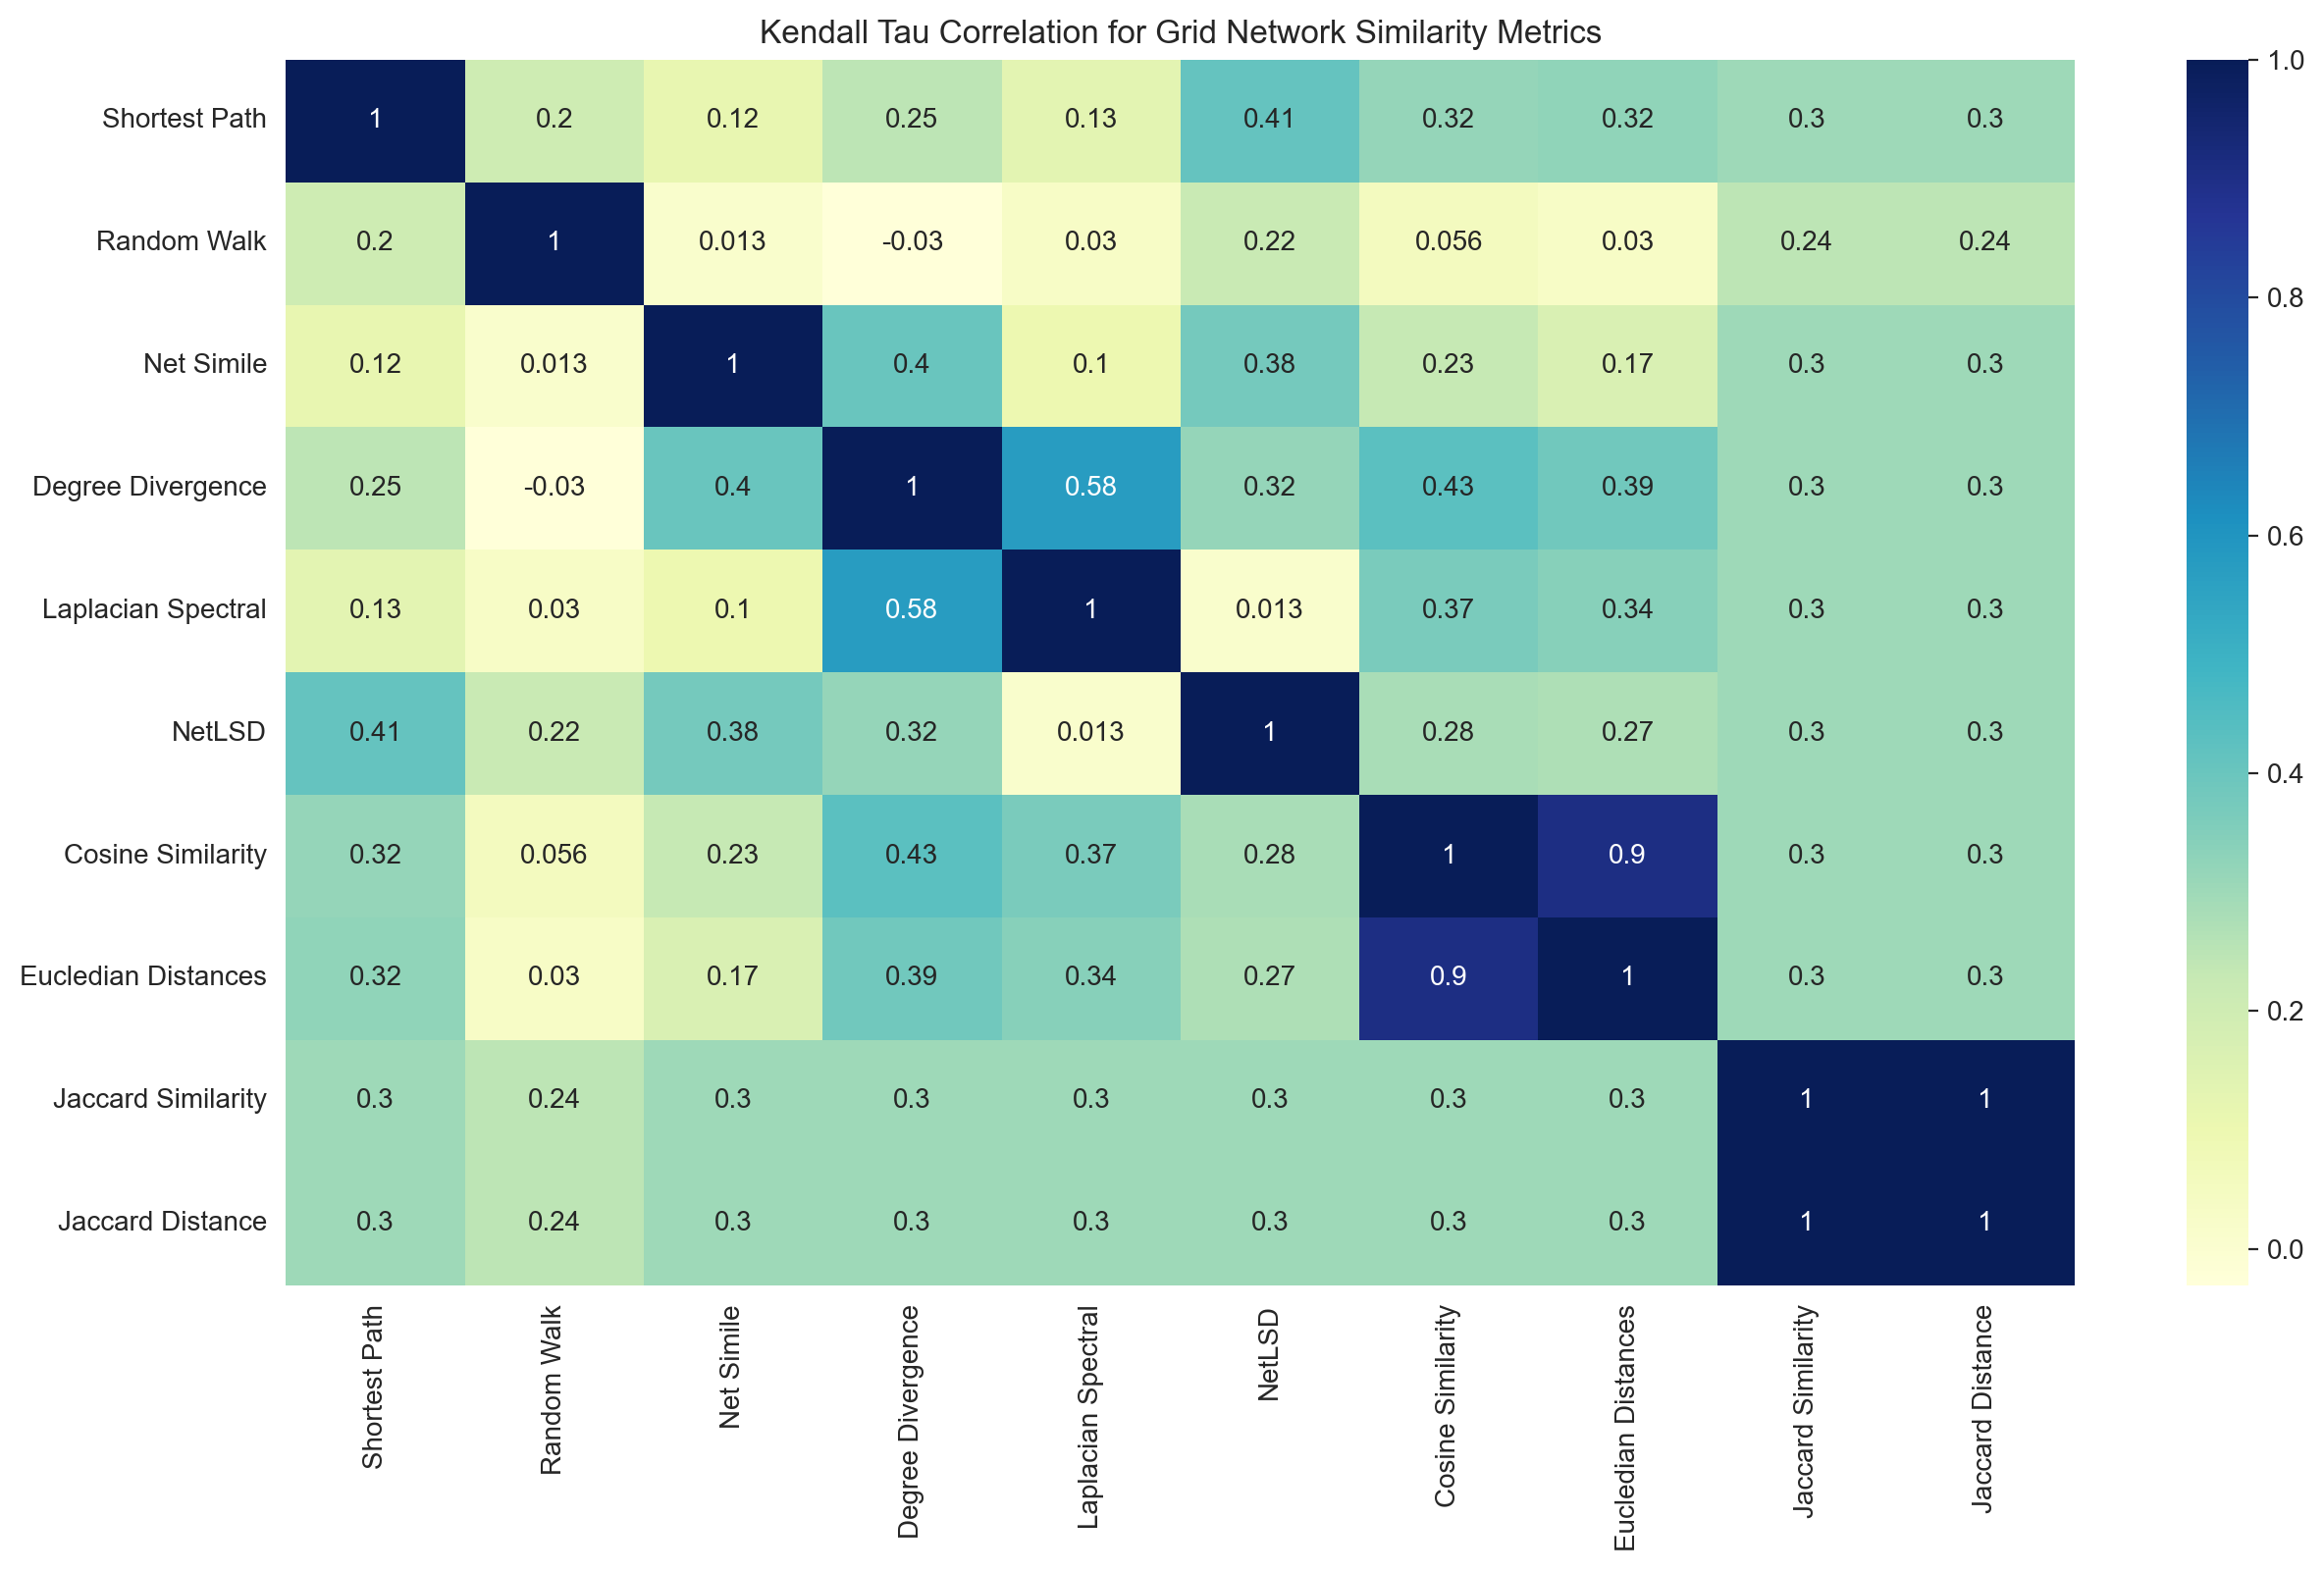
\includegraphics[width=0.85\textwidth,center]{picture/Grid/grid2.png}
\caption[Heatmap showing Kendall-Tau correlations between the road network similarity methods for Grid Road Networks]{Heatmap showing Kendall-Tau correlations between the road network similarity methods when the road network: District of Columbia was used as the reference network.}
\label{fig:network ranking}
\end{figure}

Each square illustrates the relationship between the variables on each axis. Correlation values range from 0 to 1. Values close to zero indicate that there is no linear relationship between the two variables. The closer the correlation is to one, the more positively correlated they are; that is, as one increases, so does the other, and the closer to one, the stronger the relationship. A correlation closer to 0 is similar, but instead of both variables increasing, one variable decreases as the other increases. The diagonals are all 1/dark blue because those squares are perfectly correlating each variable to itself. For the rest, the higher the correlation between the two variables, the larger the number and the darker the color. Because the same two variables are paired together in those squares, the plot is also symmetrical about the diagonal.

The Kendall-Tau distances between the scores produced by the different methods when comparing road networks similar to the reference network with a Grid pattern are shown in figure \ref{fig:network ranking}. When both the Jaccard Distance and the Jaccard Similarity are used, the results show a positive correlation of 1. This is to be expected given that the Jaccard Distance is thought to be complementary to the Jaccard Similarity, which is obtained by subtracting the Jaccard coefficient from 1. With a correlation of 0.9, the methods cosine similarity and euclidean distance also behave similarly. As shown in table \ref{tab:Road Network Similarity Methods}, both methods are vector-based and operate at the micro level. This implies that when calculating vector-based similarity on road networks at the Micro-level, either of the two methods could be used. However, there is a pronounced weaker correlation between the other methods because the level of the network they operate on and the type of comparison they use are different.

Next, the methods are clustered using complete linkage hierarchical clustering on the pairwise Kendall Tau distances, as one of the goals of using this approach is to determine whether certain network similarity methods are associated with each other. The dendrogram results are presented in the appendix section.

Finally, we can conclude that the methods operate independently of the road network pattern, but rather on the topological characteristics that define road networks as graphs.


\section{Radial Road Network Similarity Analysis}

The District of Columbia (USA) is chosen as the reference network for the Grid road similarity analysis, and the methods are used to compare the other networks to the reference network and generate a numerical similarity score. The networks are then clustered in hierarchical order. The goal is to see if certain road networks are similar to the reference network's Grid pattern, which generates a dendrogram with road network patterns that are similar to the reference road network pattern. The results for this analysis are presented in Figure \ref{fig:Hierarchical Clustering Dendrogram for Radial Road Networking Similarity}.

\begin{figure}[!ht]
\centering
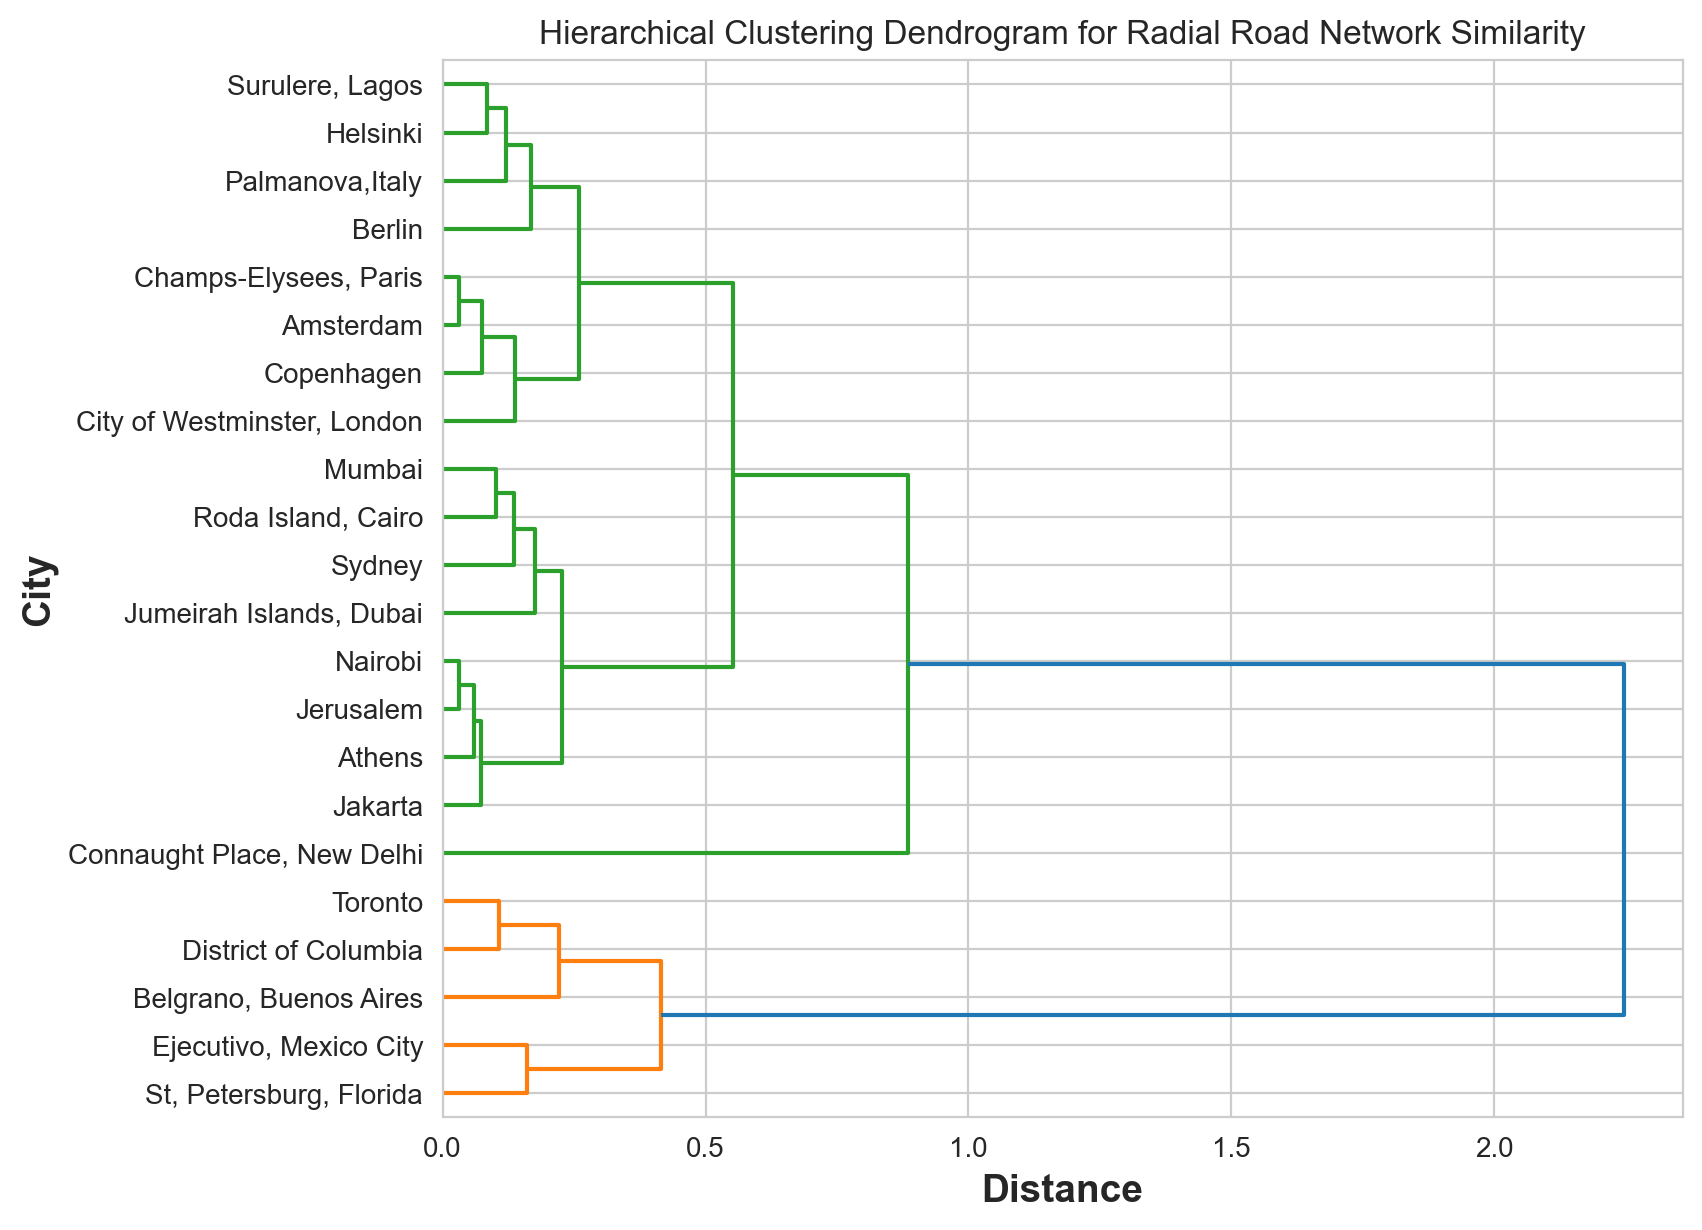
\includegraphics[width=0.75\textwidth,center]{picture/Radial/radial_dendrogram2.png}
\caption[Hierarchical Clustering Dendrogram for Radial Road Networking Similarity]{Hierarchical Clustering Dendrogram for Radial Road Networking Similarity}
\label{fig:Hierarchical Clustering Dendrogram for Radial Road Networking Similarity}
\end{figure}

Figure \ref{fig:Hierarchical Clustering Dendrogram for Radial Road Networking Similarity} presents the dendrogram obtained from the cluster analysis. The dendrogram  is interpreted using two criterias. First, a branch or cluster that includes the reference network. Second, the arrangement of the clusters which tells us the road networks that are most similar to each other, as the height of the cluster measured in distance, indicates how similar or different the road networks are from each other. The greater the distance, the greater the difference. 

For the first criteria, two major clusters (Green and Orange) can be observed from the dendrogram's structure except for the outlier; berlin road network (Blue). Looking at the green cluster, the road network for the cities Ejecutivo and Toronto lie near the reference network: District of Columbia (USA) in one adjacent cluster and are later grouped as a single cluster which indicates that this cities are the most pronounced grid-like structure similar to the reference network. 

Interpreting the dendrogram using the second criteria, the road networks for the cities Champs-Elysees, Paris and Amsterdam, Netherlands are said to be clustered first as they tend to have the cluster with the relatively shortest distance. Therefore they are the most similar than any other cluster of road networks at a higher level.

Initially, one will expect that the road networks within the green cluster should have similarities to the grid pattern of the reference network, likewise have clusters with the shortest distance, but by cross-checking with the similarity scores for each method included in the heatmap in figure \ref{fig:Heatmap showing the correlations for Radial Road Networks}, it is possible to identify the characteristics of each cluster and why certain clusters are grouped together.

\begin{figure}[!ht]
\centering
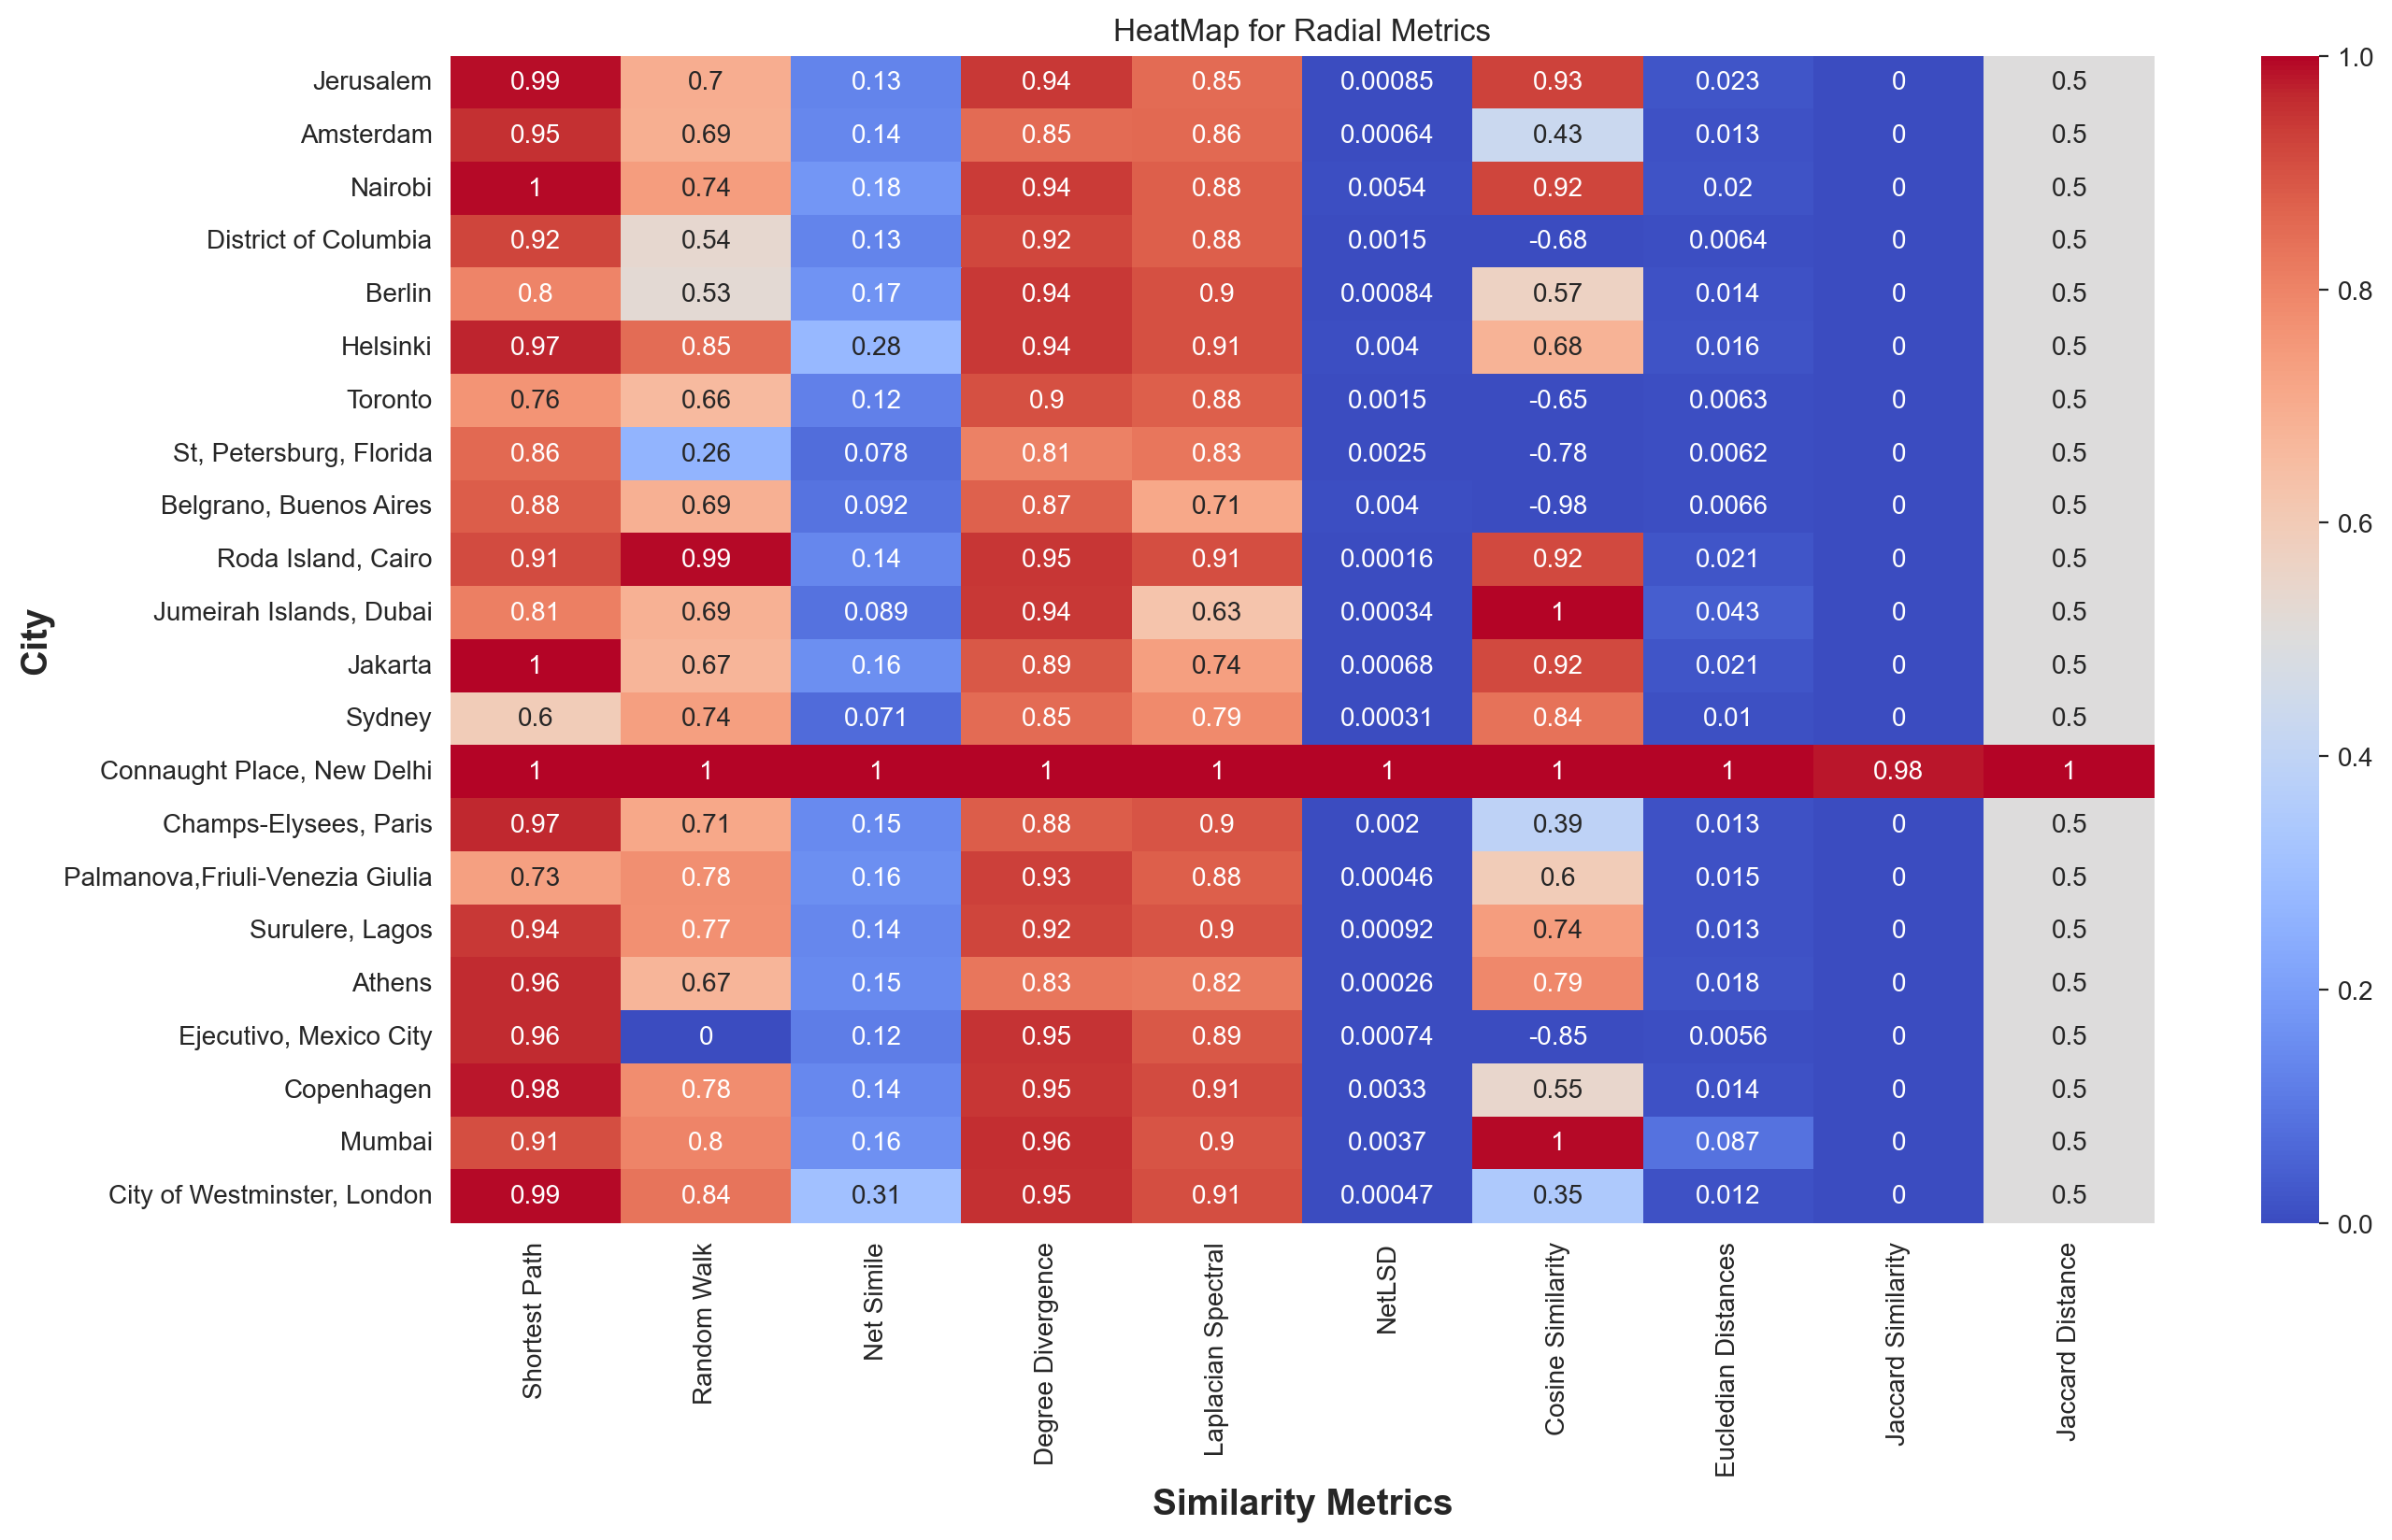
\includegraphics[width=0.85\textwidth,center]{picture/Radial/radialheatmap.png}
\caption[Heatmap showing the correlations for Radial Road Networks]{Heatmap showing the correlations between the road networks when the road network: District of Columbia was used as the reference network.}
\label{fig:Heatmap showing the correlations for Radial Road Networks}
\end{figure}


Furthermore, dendrograms only tell us a little bit about the similarities of road networks based on the clusers generated. The dendrogram clearly depicts a different picture, with some road networks grouped differently (see how the distribution of the road networks is mixed). For example, St. Petersburg, Florida, which is considered to be among the most similar to the reference network based on the similarity scores in figure \ref{fig:Heatmap showing the correlations for Radial Road Networks}, is later combined with the clusters of Ejecutivo, Toronto, and the District of Columbia (USA). As the dendrogram results are not intuitive, it is not suitable for interpreting the similarity results. Further analysis or another alternative to visualize the results of the similar scores is recommended.

In addition, dendrograms only tell us a bit in terms similarities of road networks based on the clusers generated. The dendrogram clearly shows a different picture, where some of the road networks are grouped differently (see how the distribution of the road networks is mixed). For example, St, Petersburg, Florida which from the similarity scores in figure \ref{fig:Heatmap showing the correlations for Radial Road Networks} considered to be amongst the most similar to the reference network is later put together with cluster of Ejecutivo, Toronto and the District of Columbia (USA). Further analysis is recommended or another alternative to visualize the results of the similar scores is recommended as the dendrogram results are not intuitive, thus making it not suitable for interpreting the similarity results.

To find methods that behave similarly, the pairwise Kendall-Tau distance between each pair of methods is calculated first, followed by a complete-linkage hierarchical clustering because it produces a dendrogram with many small clusters, which provides insight into which groups of methods are closely correlated.

\begin{figure}[!ht]
\centering
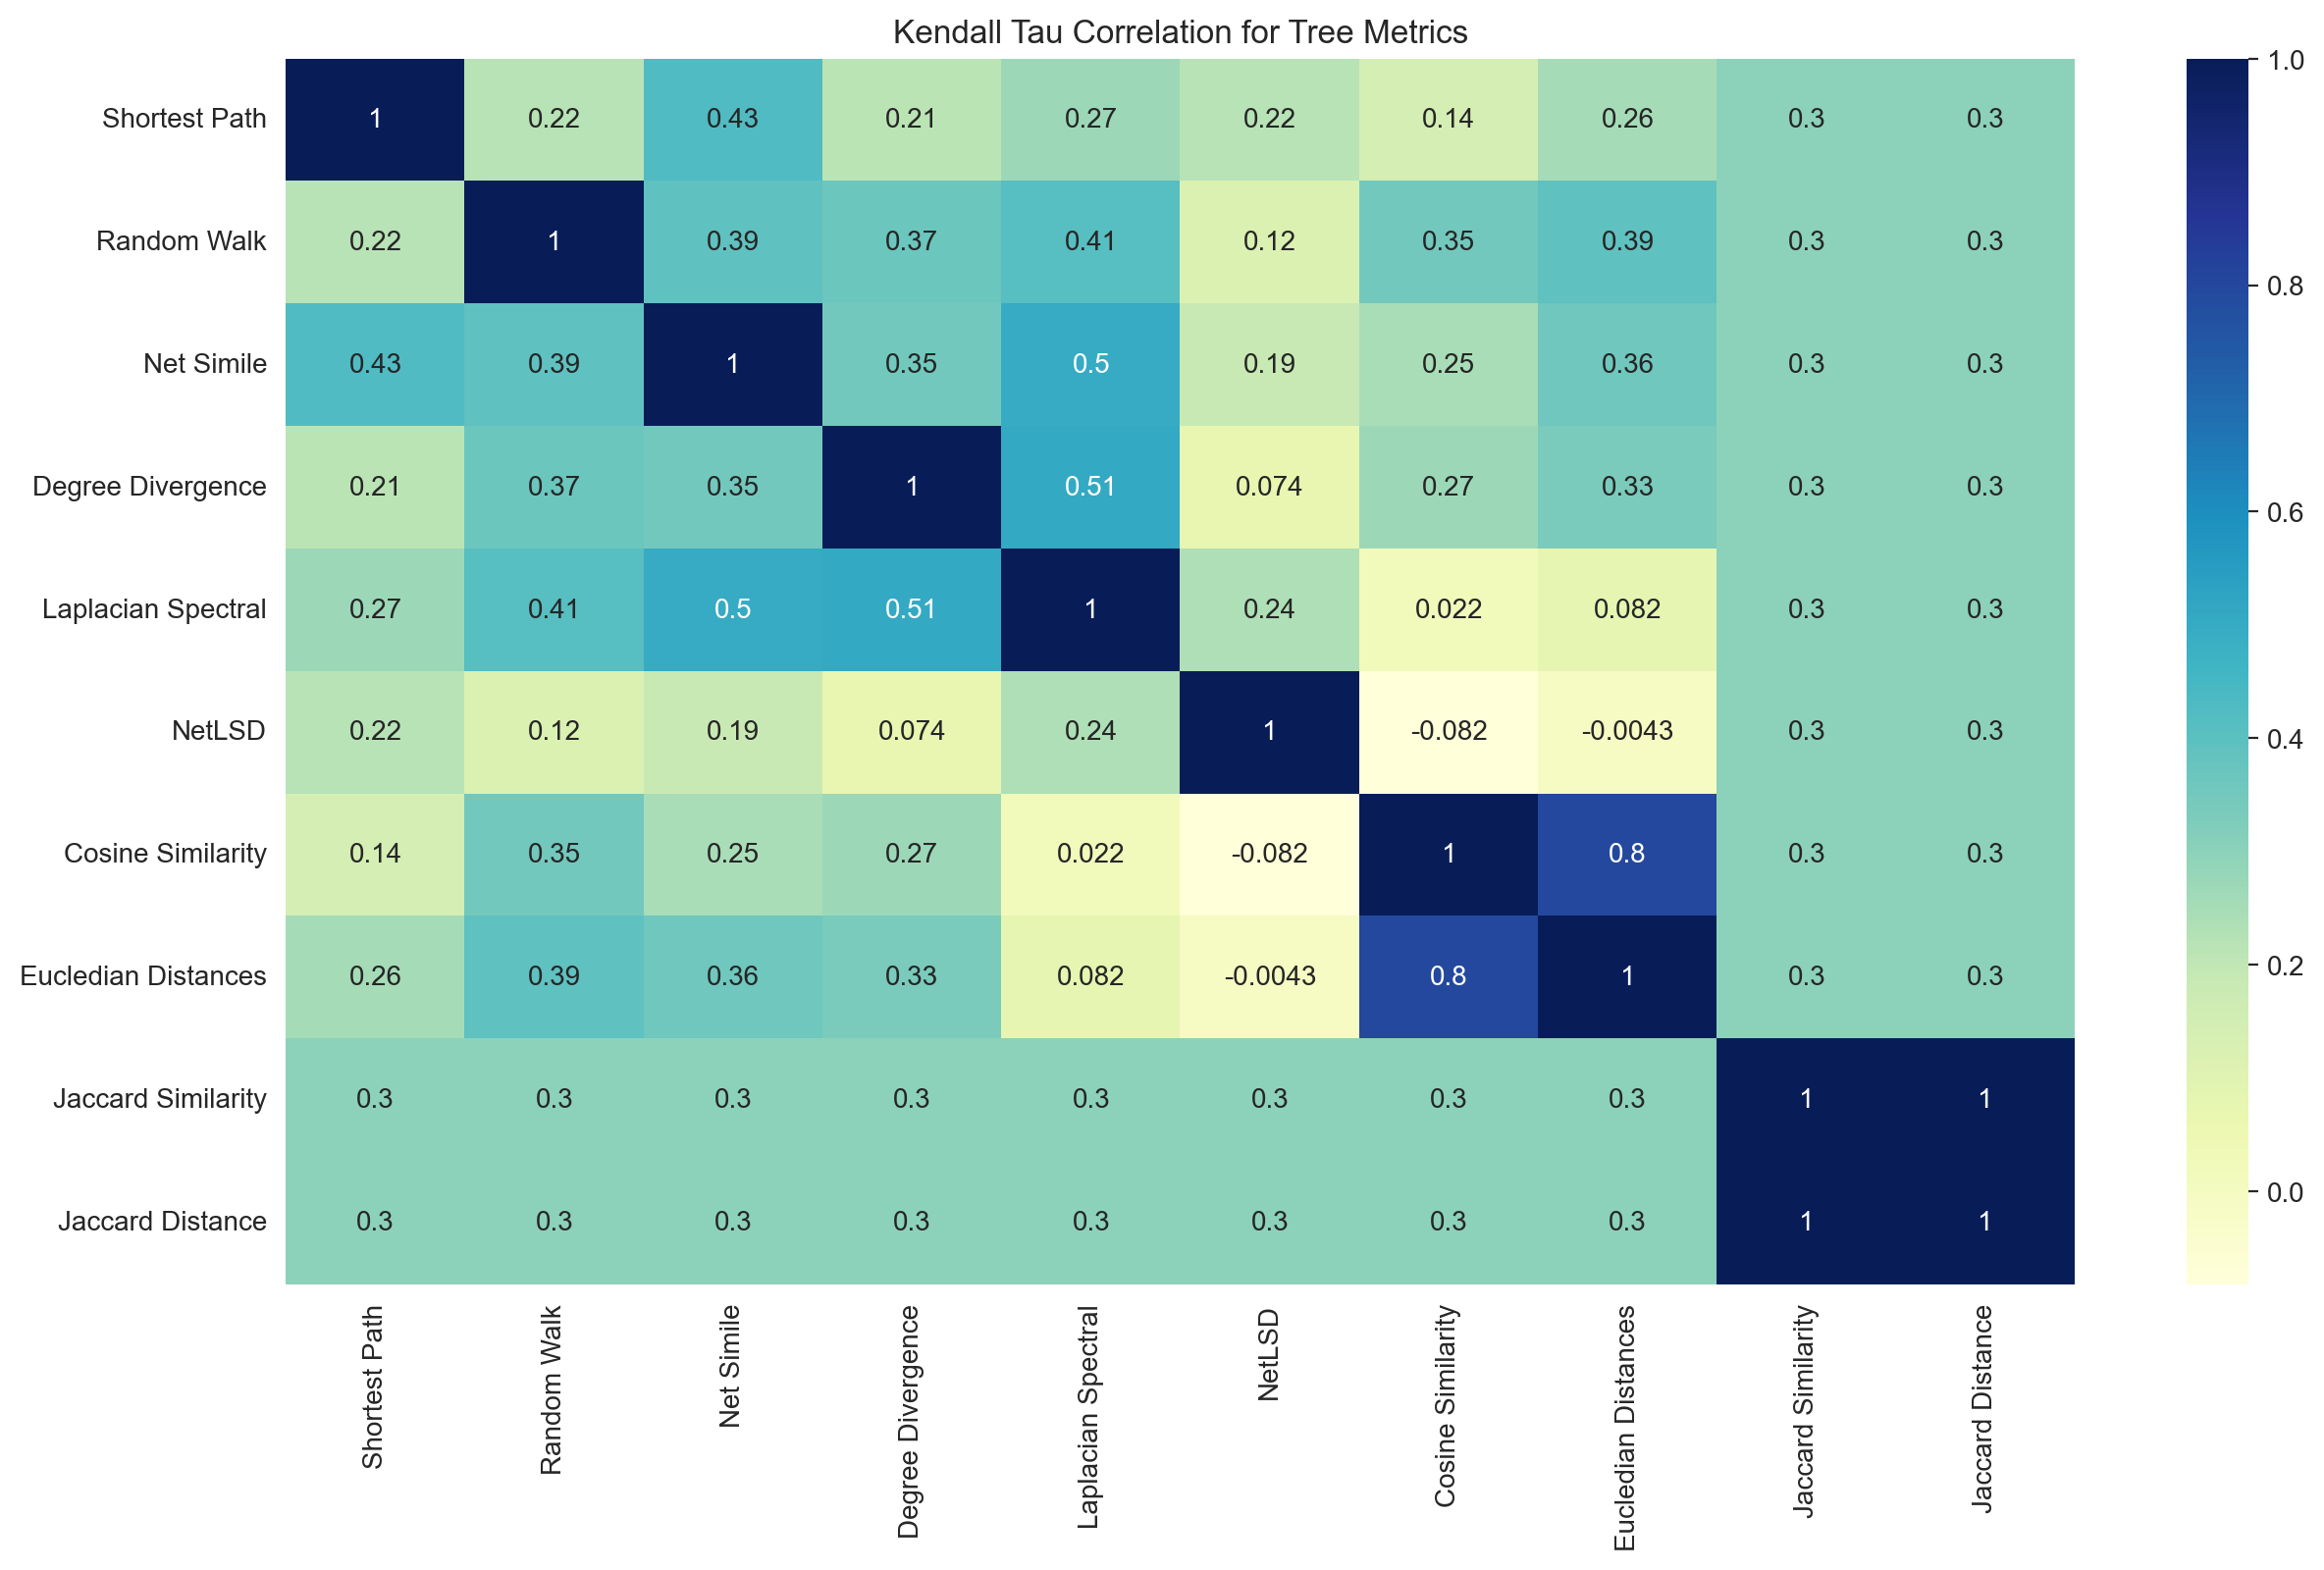
\includegraphics[width=0.85\textwidth,center]{picture/Radial/radial2.png}
\caption[Heatmap showing Kendall-Tau correlations between the road network similarity methods for Radial Road Networks]{Heatmap showing Kendall-Tau correlations between the road network similarity methods when the road network: District of Columbia was used as the reference network.}
\label{fig:network ranking radial}
\end{figure}

Each square illustrates the relationship between the variables on each axis. Correlation values range from 0 to 1. Values close to zero indicate that there is no linear relationship between the two variables. The closer the correlation is to one, the more positively correlated they are; that is, as one increases, so does the other, and the closer to one, the stronger the relationship. A correlation closer to 0 is similar, but instead of both variables increasing, one variable decreases as the other increases. The diagonals are all 1/dark blue because those squares are perfectly correlating each variable to itself. For the rest, the higher the correlation between the two variables, the larger the number and the darker the color. Because the same two variables are paired together in those squares, the plot is also symmetrical about the diagonal.

The Kendall-Tau distances between the scores produced by the different methods when comparing road networks similar to the reference network with a Grid pattern are shown in figure \ref{fig:network ranking radial}. When both the Jaccard Distance and the Jaccard Similarity are used, the results show a positive correlation of 1. This is to be expected given that the Jaccard Distance is thought to be complementary to the Jaccard Similarity, which is obtained by subtracting the Jaccard coefficient from 1. With a correlation of 0.9, the methods cosine similarity and euclidean distance also behave similarly. As shown in table \ref{tab:Road Network Similarity Methods}, both methods are vector-based and operate at the micro level. This implies that when calculating vector-based similarity on road networks at the Micro-level, either of the two methods could be used. However, there is a pronounced weaker correlation between the other methods because the level of the network they operate on and the type of comparison they use are different.

Next, the methods are clustered using complete linkage hierarchical clustering on the pairwise Kendall Tau distances, as one of the goals of using this approach is to determine whether certain network similarity methods are associated with each other. The dendrogram results are presented in the appendix section.

Finally, we can conclude that the methods operate independently of the road network pattern, but rather on the topological characteristics that define road networks as graphs.


\section{Tree Road Network Similarity Analysis}
\section{Linear Road Network Similarity Analysis}
\section{Cul de Sac Road Network Similarity Analysis}
